\section{Results}

In this chapter, we will go over the results of the experiments described in the chapter \ref{sec:experiments}. All the box plots in this chapter were generated using \citep{matplotlib}.

\subsection{Experiment 1}

The results of each run for this experiment are shown in table \ref{tab:experiment1}.

\begin{table}[!htbp]
    \centering
    \resizebox{\textwidth}{!}{
        \begin{tabular}{|l|l|l|l|l|l|l|l|l|l|l|l|}
        \hline
            Experiment 1 & RP & NN & TBGP & CGP & GBGP & SBGP & LGP & MEP & GEP & GE & SGE \\ [0.5ex] \hline\hline
            Run 1 & 3,522340 & 1,309740 & 0,646583 & 0,646583 & 0,646583 & 0,614923 & 0,630262 & 0,646583 & 1,707730 & 0,546613 & 0,646583 \\ \hline
            Run 2 & 3,408310 & 1,383550 & 0,834508 & 0,646583 & 0,646583 & 0,646583 & 0,646583 & 0,646583 & 0,646583 & 0,646583 & 0,646583 \\ \hline
            Run 3 & 3,194160 & 1,446880 & 0,646583 & 0,646583 & 0,646583 & 0,646583 & 0,646583 & 0,646583 & 0,617624 & 0,646583 & 0,646583 \\ \hline
            Run 4 & 3,116790 & 1,371300 & 0,646583 & 0,646583 & 0,564781 & 0,646583 & 0,646583 & 0,646583 & 0,646583 & 0,646583 & 0,646583 \\ \hline
            Run 5 & 3,592520 & 1,075420 & 0,646583 & 0,646583 & 0,646583 & 0,646583 & 0,646583 & 0,646583 & 0,646583 & 0,646583 & 0,646583 \\ \hline
            Run 6 & 3,567540 & 1,393190 & 0,646583 & 0,646583 & 0,646583 & 0,646583 & 0,646583 & 0,646583 & 0,646583 & 0,646583 & 0,646583 \\ \hline
            Run 7 & 3,723640 & 0,879862 & 0,646583 & 0,646583 & 0,646583 & 0,646583 & 0,646583 & 0,646583 & 0,646583 & 0,646583 & 0,639912 \\ \hline
            Run 8 & 3,450970 & 1,465860 & 0,646583 & 0,646583 & 0,646583 & 0,646583 & 0,646583 & 0,646583 & 0,778408 & 0,646583 & 0,646583 \\ \hline
            Run 9 & 3,656000 & 0,937334 & 0,601758 & 0,646583 & 0,646583 & 1,972790 & 0,646583 & 0,646583 & 0,646583 & 0,646583 & 0,646583 \\ \hline
            Run 10 & 3,531370 & 1,102690 & 0,630262 & 0,646583 & 0,606905 & 0,587223 & 0,646583 & 0,646583 & 0,646583 & 0,646583 & 0,646583 \\ \hline
        \end{tabular}
    }
    \caption{Experiment 1 - table results}
    \label{tab:experiment1}
\end{table}

A boxplot diagram of these results is shown in figure \ref{fig:experiment1}.

\begin{figure}[!htbp]
	\centering
	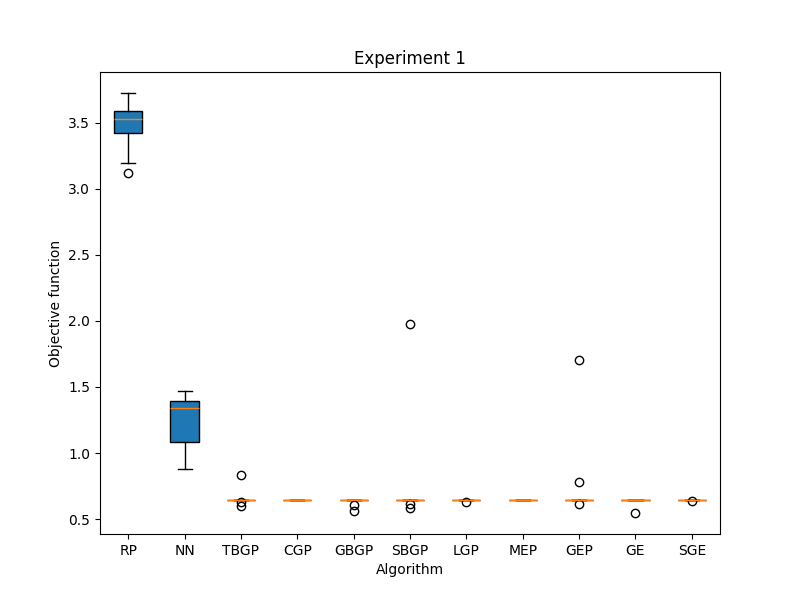
\includegraphics[scale=0.7]{../images/experiment1.png}
	\caption{Experiment 1 - boxplot results}
    \label{fig:experiment1}
\end{figure}

The boxplot diagram suggests that all the algorithms outperformed the baseline. To check this hypothesis, a t-test \citep{walpole} was performed, and the results are shown in the table \ref{tab:experiment1_stat}. All p-values are less than $0.05$, indicating that all the algorithms outperformed the baseline significantly.

\begin{table}[!htbp]
    \begin{center}
        \begin{tabular}{|l|l|} 
         \hline
            Algorithm & t-test p-value \\ [0.5ex] \hline\hline
            NN & 3.153161e-15 \\
            \hline
            TBGP & 9.251763e-20 \\
            \hline
            CGP & 3.431261e-20 \\
            \hline
            GBGP & 3.803146e-20 \\
            \hline
            SBGP & 4.014633e-13 \\
            \hline
            LGP & 3.417902e-20 \\
            \hline
            MEP & 3.431261e-20 \\
            \hline
            GEP & 1.566342e-14 \\
            \hline
            GE & 4.082947e-20 \\
            \hline
            SGE & 3.420502e-20 \\
            \hline
        \end{tabular}
    \end{center}
    \caption{Experiment 1 - t-test p-values}
\label{tab:experiment1_stat}
\end{table}

\subsection{Experiment 2}

The results of each run for this experiment are shown in table \ref{tab:experiment2}.

\begin{table}[!htbp]
    \centering
    \resizebox{\textwidth}{!}{
        \begin{tabular}{|l|l|l|l|l|l|l|l|l|l|l|l|}
        \hline
            Experiment 2 & RP & NN & TBGP & CGP & GBGP & SBGP & LGP & MEP & GEP & GE & SGE \\ [0.5ex] \hline\hline
            Run 1 & 46,552200 & 28,160800 & 29,387600 & 29,564600 & 28,408500 & 28,197100 & 27,755200 & 29,382300 & 27,981000 & 27,941300 & 28,700600 \\ \hline
            Run 2 & 47,323500 & 28,678000 & 26,925900 & 28,058400 & 28,150900 & 28,052900 & 30,245300 & 31,617800 & 28,511000 & 31,177500 & 29,047800 \\ \hline
            Run 3 & 45,785300 & 29,390100 & 28,195500 & 27,863900 & 27,285300 & 27,939100 & 27,886900 & 27,883500 & 28,137000 & 27,916800 & 28,153300 \\ \hline
            Run 4 & 45,666100 & 28,852300 & 30,527100 & 28,572500 & 27,813000 & 28,105700 & 27,857200 & 28,171000 & 29,389000 & 30,569100 & 27,285300 \\ \hline
            Run 5 & 43,870700 & 30,717500 & 27,681500 & 27,835400 & 29,104600 & 28,351400 & 28,148400 & 30,048700 & 29,445700 & 27,966500 & 29,924900 \\ \hline
            Run 6 & 45,824500 & 30,254200 & 29,020600 & 29,273000 & 28,301500 & 29,056500 & 28,153100 & 30,026000 & 28,468800 & 28,800800 & 28,050900 \\ \hline
            Run 7 & 46,213200 & 28,858000 & 28,531900 & 29,201200 & 28,424300 & 27,871500 & 28,195800 & 29,034100 & 28,967800 & 28,601500 & 29,536000 \\ \hline
            Run 8 & 43,138800 & 30,106800 & 30,164800 & 28,621500 & 29,589600 & 27,348800 & 27,265700 & 30,964000 & 29,774800 & 27,568200 & 29,230600 \\ \hline
            Run 9 & 45,130700 & 30,389200 & 29,591900 & 28,395100 & 27,890800 & 29,214000 & 28,275100 & 30,035800 & 28,389100 & 29,973300 & 29,592700 \\ \hline
            Run 10 & 45,388900 & 30,492900 & 27,314800 & 29,691700 & 26,729000 & 28,670100 & 28,363400 & 29,468400 & 29,396600 & 27,889900 & 29,076100 \\ \hline
        \end{tabular}
    }
    \caption{Experiment 2 - table results}
    \label{tab:experiment2}
    \end{table}
    
A boxplot diagram of these results is shown in figure \ref{fig:experiment2}. This diagram suggests that all the algorithms outperformed the baseline.

\begin{figure}[!htbp]
    \centering
    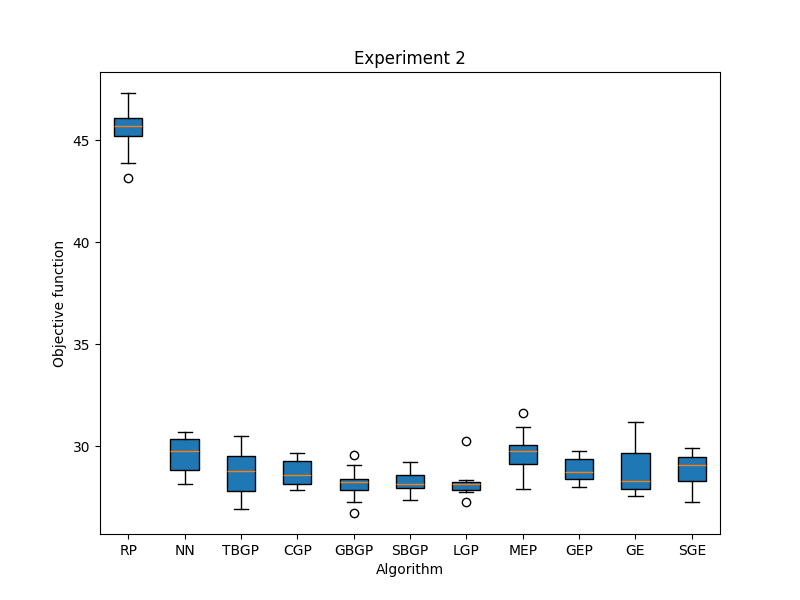
\includegraphics[scale=0.7]{../images/experiment2.png}
    \caption{Experiment 2 - boxplot results}
    \label{fig:experiment2}
\end{figure}

The results of the t-test are shown in the table \ref{tab:experiment2_stat}. All p-values are less than $0.05$, indicating that all the algorithms outperformed the baseline significantly.
    
\begin{table}[!htbp]
    \begin{center}
        \begin{tabular}{|l|l|} 
         \hline
            Algorithm & t-test p-value \\ [0.5ex] \hline\hline
            NN & 1.528360e-17 \\
            \hline
            TBGP & 5.253220e-17 \\
            \hline
            CGP & 1.384135e-18 \\
            \hline
            GBGP & 1.865969e-18 \\
            \hline
            SBGP & 4.244256e-19 \\
            \hline
            LGP & 1.491073e-18 \\
            \hline
            MEP & 8.980485e-17 \\
            \hline
            GEP & 1.102975e-18 \\
            \hline
            GE & 9.547008e-17 \\
            \hline
            SGE & 3.695756e-18 \\
            \hline
        \end{tabular}
    \end{center}
    \caption{Experiment 2 - t-test p-values}
\label{tab:experiment2_stat}
\end{table}

\subsection{Experiment 3}

The results of each run for this experiment are shown in table \ref{tab:experiment3}.

\begin{table}[!htbp]
    \centering
    \resizebox{\textwidth}{!}{
        \begin{tabular}{|l|l|l|l|l|l|l|l|l|l|l|l|}
        \hline
            Experiment 3 & RP & NN & TBGP & CGP & GBGP & SBGP & LGP & MEP & GEP & GE & SGE \\ [0.5ex] \hline\hline
            Run 1 & 398,571000 & 142,231000 & 76,278000 & 78,850600 & 81,262600 & 86,935900 & 79,845300 & 84,390900 & 76,763900 & 441,695000 & 79,117400 \\ \hline
            Run 2 & 404,800000 & 128,942000 & 76,804200 & 77,059900 & 79,065000 & 84,673700 & 82,811300 & 94,337600 & 81,856200 & 454,021000 & 79,157200 \\ \hline
            Run 3 & 430,162000 & 151,423000 & 76,235200 & 77,917300 & 79,608100 & 82,899400 & 77,423000 & 441,235000 & 75,788100 & 87,985100 & 78,712400 \\ \hline
            Run 4 & 415,491000 & 115,145000 & 72,214100 & 78,081400 & 81,774500 & 86,875800 & 79,168600 & 446,631000 & 75,535700 & 105,626000 & 79,567700 \\ \hline
            Run 5 & 455,789000 & 203,372000 & 77,203800 & 77,550100 & 78,552700 & 80,235500 & 75,237900 & 79,520600 & 77,470100 & 454,021000 & 78,526300 \\ \hline
            Run 6 & 401,102000 & 160,634000 & 77,159400 & 78,586300 & 78,183300 & 81,754000 & 78,635600 & 441,098000 & 83,878700 & 454,021000 & 80,165400 \\ \hline
            Run 7 & 425,054000 & 89,669000 & 76,210700 & 79,521800 & 82,321900 & 82,172300 & 75,663500 & 454,021000 & 78,505400 & 78,534200 & 90,099400 \\ \hline
            Run 8 & 433,056000 & 110,014000 & 77,293000 & 81,825500 & 79,535300 & 85,812500 & 84,361100 & 90,789100 & 78,391500 & 454,021000 & 96,145100 \\ \hline
            Run 9 & 386,019000 & 139,035000 & 79,829400 & 82,854100 & 77,976900 & 90,877700 & 79,812100 & 77,195200 & 77,968100 & 78,332800 & 85,831700 \\ \hline
            Run 10 & 436,368000 & 159,275000 & 75,827800 & 82,321800 & 79,608100 & 81,819700 & 80,073600 & 80,687600 & 78,212300 & 78,896900 & 82,356900 \\ \hline
        \end{tabular}
    }
    \caption{Experiment 3 - table results}
    \label{tab:experiment3}
\end{table}

A boxplot diagram of these results is shown in figure \ref{fig:experiment3}. This diagram suggests that all the algorithms outperformed the baseline, with the exception of MEP and GE. While the means for these algorithms were lower than the means for RP, they did have some bad runs, possibly indicating that these algorithms could scale poorly with the number of regression algorithms to train simultaneously, as this experiment had the largest number of machines.

\begin{figure}[!htbp]
	\centering
	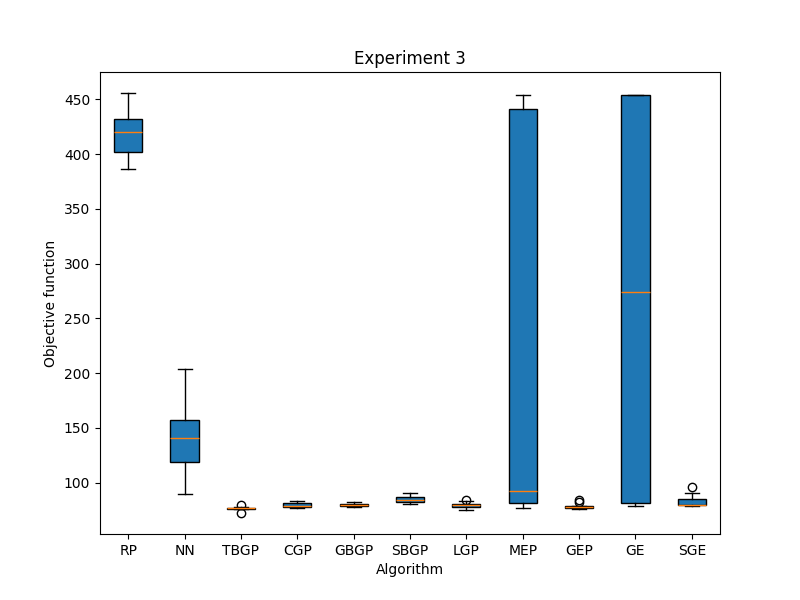
\includegraphics[scale=0.7]{../images/experiment3.png}
	\caption{Experiment 3 - boxplot results}
    \label{fig:experiment3}
\end{figure}

The results of the t-test are shown in the table \ref{tab:experiment3_stat}. All p-values are less than $0.05$, indicating that all the algorithms, even MEP and GE, outperformed the baseline significantly.

\begin{table}[!htbp]
    \begin{center}
        \begin{tabular}{|l|l|} 
         \hline
            Algorithm & t-test p-value \\ [0.5ex] \hline\hline
            NN & 8.309557e-15 \\
            \hline
            TBGP & 6.849891e-21 \\
            \hline
            CGP & 8.145383e-21 \\
            \hline
            GBGP & 7.941702e-21 \\
            \hline
            SBGP & 1.192731e-20 \\
            \hline
            LGP & 8.675050e-21 \\
            \hline
            MEP & 5.045305e-03 \\
            \hline
            GEP & 8.074380e-21 \\
            \hline
            GE & 2.511749e-02 \\
            \hline
            SGE & 1.770743e-20 \\
            \hline
        \end{tabular}
    \end{center}
    \caption{Experiment 3 - t-test p-values}
\label{tab:experiment3_stat}
\end{table}

\subsection{Experiment 4}

The results of each run for this experiment are shown in table \ref{tab:experiment4}.

\begin{table}[!htbp]
    \centering
    \resizebox{\textwidth}{!}{
        \begin{tabular}{|l|l|l|l|l|l|l|l|l|l|l|l|}
        \hline
            Experiment 4 & RP & NN & TBGP & CGP & GBGP & SBGP & LGP & MEP & GEP & GE & SGE \\ [0.5ex] \hline\hline
            Run 1 & 306,095000 & 170,278000 & 133,797000 & 131,288000 & 133,343000 & 130,724000 & 132,240000 & 142,987000 & 133,701000 & 131,308000 & 137,616000 \\ \hline
            Run 2 & 295,783000 & 156,802000 & 128,192000 & 149,564000 & 132,408000 & 130,724000 & 131,827000 & 159,583000 & 129,635000 & 142,048000 & 131,246000 \\ \hline
            Run 3 & 299,499000 & 164,053000 & 130,144000 & 131,210000 & 134,904000 & 133,533000 & 131,062000 & 154,665000 & 134,741000 & 133,383000 & 129,637000 \\ \hline
            Run 4 & 297,632000 & 160,097000 & 131,355000 & 157,199000 & 131,476000 & 132,535000 & 131,370000 & 183,651000 & 134,635000 & 131,226000 & 132,113000 \\ \hline
            Run 5 & 307,868000 & 163,259000 & 132,369000 & 134,472000 & 131,259000 & 132,027000 & 130,805000 & 130,391000 & 134,300000 & 132,085000 & 130,736000 \\ \hline
            Run 6 & 302,434000 & 139,903000 & 131,085000 & 133,277000 & 131,682000 & 135,446000 & 129,909000 & 134,296000 & 134,202000 & 138,143000 & 130,574000 \\ \hline
            Run 7 & 310,132000 & 154,048000 & 142,569000 & 133,573000 & 131,168000 & 133,553000 & 137,309000 & 138,107000 & 138,959000 & 136,530000 & 131,900000 \\ \hline
            Run 8 & 306,348000 & 151,054000 & 135,071000 & 133,601000 & 130,485000 & 133,604000 & 132,904000 & 143,358000 & 144,316000 & 128,125000 & 137,641000 \\ \hline
            Run 9 & 298,524000 & 139,714000 & 137,647000 & 132,862000 & 132,862000 & 133,070000 & 131,410000 & 131,103000 & 135,322000 & 136,151000 & 134,385000 \\ \hline
            Run 10 & 302,474000 & 158,785000 & 131,416000 & 129,397000 & 131,435000 & 131,682000 & 128,509000 & 132,378000 & 136,622000 & 172,459000 & 135,120000 \\ \hline
        \end{tabular}
    }
    \caption{Experiment 4 - table results}
    \label{tab:experiment4}
\end{table}

A boxplot diagram of these results is shown in figure \ref{fig:experiment4}. This diagram suggests that all the algorithms outperformed the baseline.

\begin{figure}[!htbp]
	\centering
	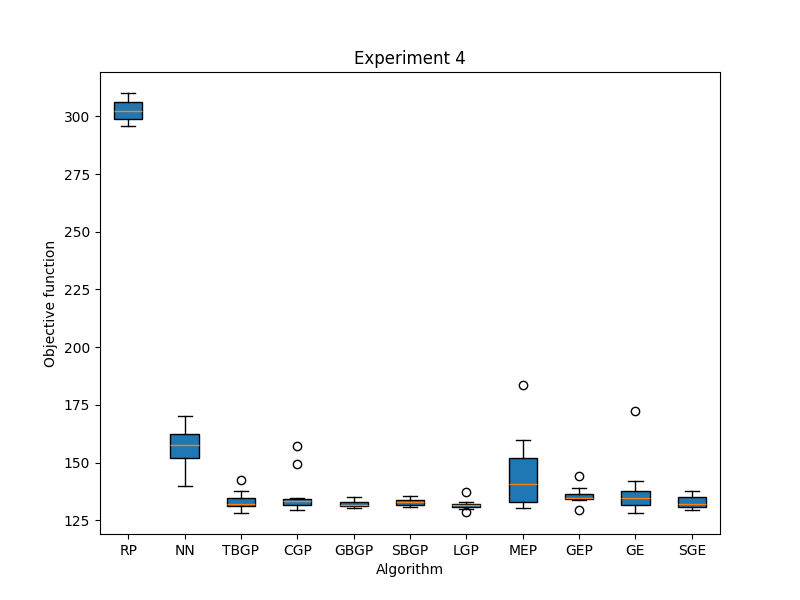
\includegraphics[scale=0.7]{../images/experiment4.png}
	\caption{Experiment 4 - boxplot results}
    \label{fig:experiment4}
\end{figure}

The results of the t-test are shown in the table \ref{tab:experiment4_stat}. All p-values are less than $0.05$, indicating that all the algorithms outperformed the baseline significantly.

\begin{table}[!htbp]
    \begin{center}
        \begin{tabular}{|l|l|} 
         \hline
            Algorithm & t-test p-value \\ [0.5ex] \hline\hline
            NN & 2.144677e-19 \\
            \hline
            TBGP & 8.255094e-25 \\
            \hline
            CGP & 6.573689e-21 \\
            \hline
            GBGP & 8.684286e-27 \\
            \hline
            SBGP & 1.082375e-26 \\
            \hline
            LGP & 2.853916e-26 \\
            \hline
            MEP & 1.917750e-16 \\
            \hline
            GEP & 5.653282e-25 \\
            \hline
            GE & 1.058940e-18 \\
            \hline
            SGE & 8.519537e-26 \\
            \hline
        \end{tabular}
    \end{center}
    \caption{Experiment 4 - t-test p-values}
\label{tab:experiment4_stat}
\end{table}

\subsection{Experiment 5}

The results of each run for this experiment are shown in table \ref{tab:experiment5}. 

\begin{table}[!htbp]
    \centering
    \resizebox{\textwidth}{!}{
        \begin{tabular}{|l|l|l|l|l|l|l|l|l|l|l|l|}
        \hline
            Experiment 5 & RP & NN & TBGP & CGP & GBGP & SBGP & LGP & MEP & GEP & GE & SGE \\ [0.5ex] \hline\hline
            Run 1 & 498,021000 & 334,282000 & 284,843000 & 279,889000 & 294,719000 & 297,456000 & 287,861000 & 285,314000 & 282,517000 & 284,571000 & 274,993000 \\ \hline
            Run 2 & 496,935000 & 347,374000 & 268,641000 & 289,903000 & 284,769000 & 293,487000 & 275,373000 & 285,638000 & 285,802000 & 297,712000 & 277,462000 \\ \hline
            Run 3 & 500,548000 & 331,207000 & 280,611000 & 285,536000 & 279,026000 & 290,237000 & 287,868000 & 284,178000 & 284,524000 & 289,665000 & 275,507000 \\ \hline
            Run 4 & 514,241000 & 309,262000 & 280,538000 & 284,318000 & 283,449000 & 294,006000 & 265,770000 & 308,040000 & 269,349000 & 287,539000 & 268,799000 \\ \hline
            Run 5 & 496,808000 & 318,476000 & 271,222000 & 278,149000 & 276,546000 & 289,545000 & 285,781000 & 288,403000 & 284,525000 & 291,359000 & 269,010000 \\ \hline
            Run 6 & 498,408000 & 339,338000 & 261,601000 & 280,697000 & 285,987000 & 287,927000 & 281,340000 & 289,647000 & 286,713000 & 282,650000 & 280,829000 \\ \hline
            Run 7 & 515,917000 & 323,415000 & 266,261000 & 285,591000 & 273,531000 & 296,472000 & 298,221000 & 292,495000 & 284,976000 & 291,166000 & 279,720000 \\ \hline
            Run 8 & 497,740000 & 317,707000 & 277,294000 & 288,019000 & 286,353000 & 291,169000 & 269,855000 & 305,503000 & 286,452000 & 288,810000 & 261,809000 \\ \hline
            Run 9 & 516,560000 & 310,174000 & 271,102000 & 291,225000 & 269,259000 & 285,453000 & 290,787000 & 280,492000 & 273,917000 & 274,270000 & 273,391000 \\ \hline
            Run 10 & 513,262000 & 339,668000 & 278,854000 & 273,967000 & 281,909000 & 296,069000 & 286,594000 & 301,451000 & 276,441000 & 280,912000 & 276,351000 \\ \hline
        \end{tabular}
    }
    \caption{Experiment 5 - table results}
    \label{tab:experiment5}
\end{table}

A boxplot diagram of these results is shown in figure \ref{fig:experiment5}. This diagram suggests that all the algorithms outperformed the baseline.

\begin{figure}[!htbp]
	\centering
	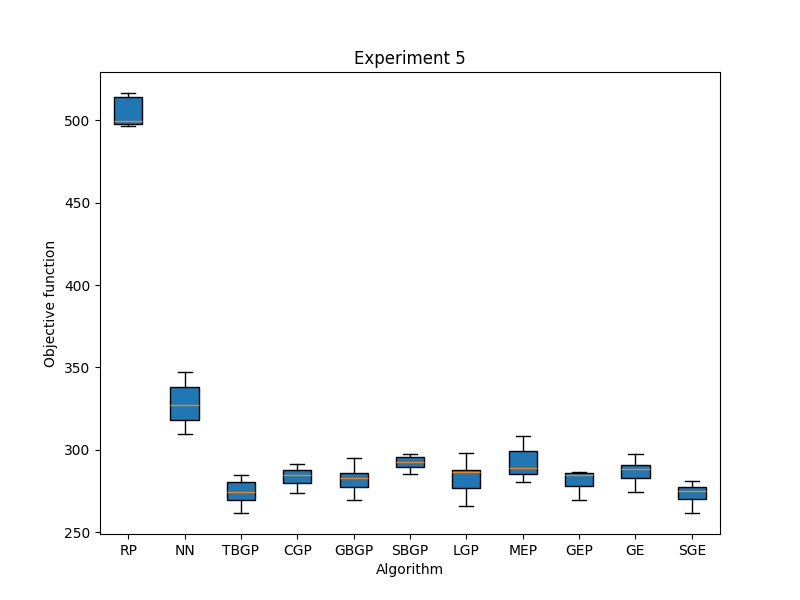
\includegraphics[scale=0.7]{../images/experiment5.png}
	\caption{Experiment 5 - boxplot results}
    \label{fig:experiment5}
\end{figure}

The results of the t-test are shown in the table \ref{tab:experiment5_stat}. All p-values are less than $0.05$, indicating that all the algorithms outperformed the baseline significantly.

\begin{table}[!htbp]
    \begin{center}
        \begin{tabular}{|l|l|} 
         \hline
            Algorithm & t-test p-value \\ [0.5ex] \hline\hline
            NN & 4.305292e-18 \\
            \hline
            TBGP & 1.369618e-22 \\
            \hline
            CGP & 4.504320e-23 \\
            \hline
            GBGP & 2.126929e-22 \\
            \hline
            SBGP & 2.541160e-23 \\
            \hline
            LGP & 3.507470e-21 \\
            \hline
            MEP & 5.156325e-21 \\
            \hline
            GEP & 6.568137e-23 \\
            \hline
            GE & 1.588308e-22 \\
            \hline
            SGE & 2.697942e-23 \\
            \hline
        \end{tabular}
    \end{center}
    \caption{Experiment 5 - t-test p-values}
\label{tab:experiment5_stat}
\end{table}

\section{Analysis of the results}

The results of the experiments were rather satisfying. On every experiment, every algorithm outperformed the baseline. This holds an even greater weight when we consider that these algorithms worked with vastly different hyperparameters. This indicates that all the concepts presented in this thesis work together fairly well, and that it is possible to use the hierarchical topology representation to solve online scheduling problems.

Another important thing to note is that, across five experiments, we were able to solve problems with completely different machine topologies and behaviors. We were able to use a single system to solve five different problems, without the need to develop anything specific for any of them. This proves that the hierarchical topology representation is immensely versatile in regards to the types of problems it can be used to solve.

\section{Examples of generated heuristics}

In this chapter, we will show the best solution across all runs in the fourth experiment, which was achieved using TBGP. To recap, the fourth experiment utilized setups and batch processing, so we can expect features related to these behaviors to be present in the genotype.

The symbolic expressions, represented as a tree where the child nodes of a node are indented with one space more than the parent node, are shown in the following figures - $O_1$ in figure \ref{fig:heuristic_01}, $M_1$ in figure \ref{fig:heuristic_02}, $M_2$ in figure \ref{fig:heuristic_03}, $M_3$ in figure \ref{fig:heuristic_04}, $M_4$ in figure \ref{fig:heuristic_05} and $M_5$ in figure \ref{fig:heuristic_06}.

Interestingly, the results show that the batch processing features were heavily utilized in online scheduling algorithms for machines, while the setup features were not utilized. This may be due to the fact that setup times did not vary between jobs, so the algorithm could not discriminate jobs by these features.

\begin{figure}[!htbp]
	\centering
	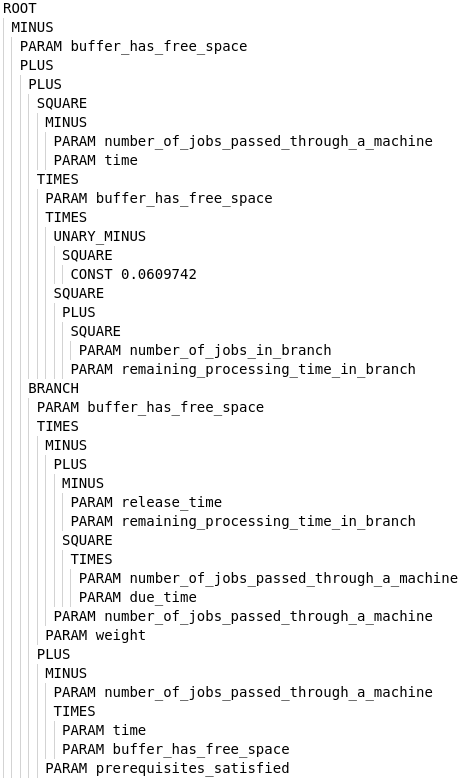
\includegraphics[scale=0.7]{../images/heuristic_01.png}
	\caption{Generated heuristics - experiment 4, $O_1$}
    \label{fig:heuristic_01}
\end{figure}

\begin{figure}[!htbp]
	\centering
	
\includegraphics[scale=0.7]{../images/heuristic_02.png}
	\caption{Generated heuristics - experiment 4, $M_1$}
    \label{fig:heuristic_02}
\end{figure}

\begin{figure}[!htbp]
	\centering
	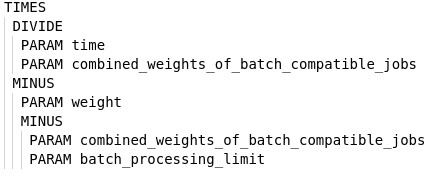
\includegraphics[scale=0.7]{../images/heuristic_03.png}
	\caption{Generated heuristics - experiment 4, $M_2$}
    \label{fig:heuristic_03}
\end{figure}

\begin{figure}[!htbp]
	\centering
	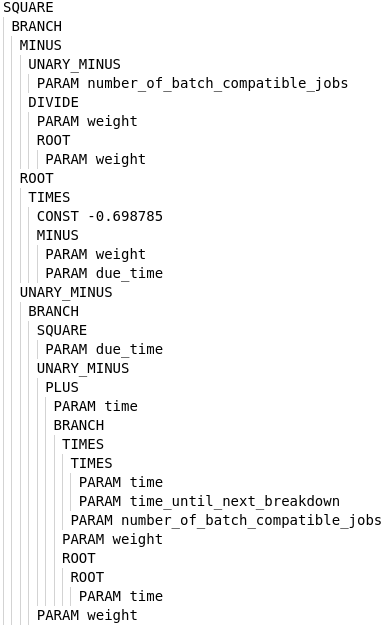
\includegraphics[scale=0.7]{../images/heuristic_04.png}
	\caption{Generated heuristics - experiment 4, $M_3$}
    \label{fig:heuristic_04}
\end{figure}

\begin{figure}[!htbp]
	\centering
	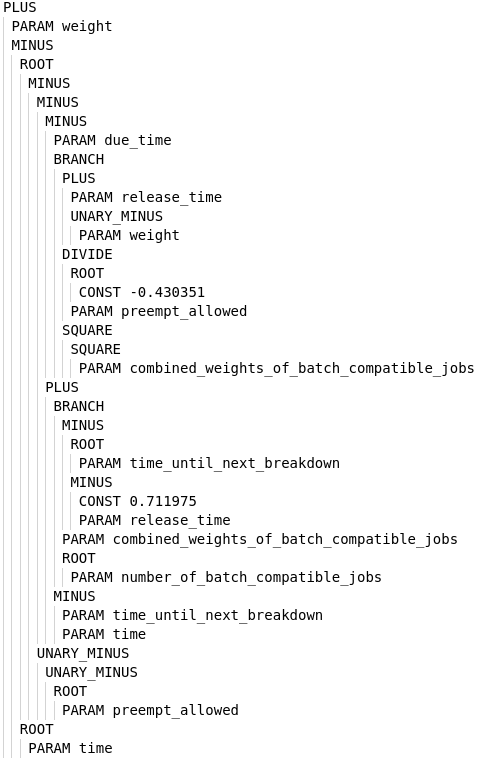
\includegraphics[scale=0.7]{../images/heuristic_05.png}
	\caption{Generated heuristics - experiment 4, $M_4$}
    \label{fig:heuristic_05}
\end{figure}

\begin{figure}[!htbp]
	\centering
	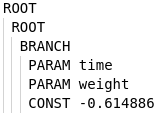
\includegraphics[scale=0.7]{../images/heuristic_06.png}
	\caption{Generated heuristics - experiment 4, $M_5$}
    \label{fig:heuristic_06}
\end{figure}